
\lecture{4}{Energy in Thermal Physics}{Qiang Zhu}{scribe-name1,2,3}
%\section{Some useful equations} % Don't be this informal in your notes!
%\begin{equation} \label{idealgas} PV = nRT = NkT \end{equation}
%\begin{equation} \label{Avogadro} N = n \times N_A \end{equation}
%\begin{equation} \label{PV-micro} PV = Nm{\overline v_x^2} = NkT \end{equation}
%\begin{equation} \label{eqpartition} U_\text{thermal} = N \cdot f \cdot \frac{1}{2}kT \end{equation}

\section{Compression Work}

\begin{equation} \label{duw5} VT^{f/2} = \textrm{const}. \end{equation}
\begin{equation} \label{duw6} V^{\gamma}P = \textrm{const}. \end{equation}
where ${\gamma}$ = $\frac{f+2}{f}$ is called adiabatic exponent.\\

{\bf Exercises}\\
(Problem 1.38):\\
Two identical bubbles rise from the bottom of a lake to its surface.\\
Bubble A rises quickly (adiabatic condition).\\
Bubble B rises slowly (isothermal condition).\\
Which buble is larger in the end?
 \\\\\\

(Problem 1.40):\\
In Lec02, we have determined that 
  \begin{equation} \frac{dP}{dz} = -\frac{mg}{kT} P \end{equation}
and obtained the pressure $P$ as a function of height as follows,
  \begin{equation} P(z) = P(0) \exp(-mgz/kT) \end{equation}

1) show that $T$ and $P$ has the following relation
  \begin{equation} \frac{dT}{dP} = \frac{2}{f+2} \frac{T}{P} \end{equation}
2) find a formula for $dT/dz$ like $dP/dz$.\\
3) estimate the temperature at the peak of Mount Everest (8848 km).\\\\\\\\\\\\\\\\\\\\\

\section{Heat Capacities}
The heat capacity of an object is the amount of heat needed to raise its temperature,
  \begin{equation} C = \frac{Q}{\Delta{T}} = \frac{\Delta{U}-W}{\Delta{T}}\end{equation}
Specific heat capacity is a more fundamental metric,
  \begin{equation} c = \frac{C}{m}. \end{equation}

There are two types of circumstances
\begin{enumerate}
\item{constant volume}, $C_V$
\item{constant pressure}, $C_P$
\end{enumerate}
Obviously, $C_P$ is more representative than $C_V$.
According to the eqipartition theorem,
  \begin{equation} C_V = \frac{\partial U}{\partial{T}} 
                       = \frac{\partial} {\partial{T}}(\frac {NfkT}{2})
                       = \frac{Nfk}{2}
  \end{equation}
Under constant pressure,
  \begin{equation} C_P = \frac{\partial (U-W)} {\partial{T}} 
                       = \frac{\partial} {\partial{T}}(\frac {NfkT}{2}) - \frac{\partial W}{\partial{T}}
  \end{equation}
  \begin{equation}
                \frac{\partial W}{\partial{T}} = -P\frac{\partial V}{\partial T} 
                                                = -P\frac{\partial (NkT/P)}{\partial T} 
                                                = -Nk
  \end{equation}
therefore, 
  \begin{equation} C_P = C_V + Nk. \end{equation}
using ideal gas law.\\\\

{\bf Discussions}: 
\begin{enumerate}
\item{What's the relation between $C_V$ and $C_P$ for solids?}
\item{$C_V$ of 1 mole of H$_2$ gas as a function of temperature (see Figure \ref{cv-h2})}
\item{$C_P$ of 1 mole of elemental solids as a function of temperature (see Figure \ref{cv-metal})}
\end{enumerate}

\begin{figure}[h]
\centering
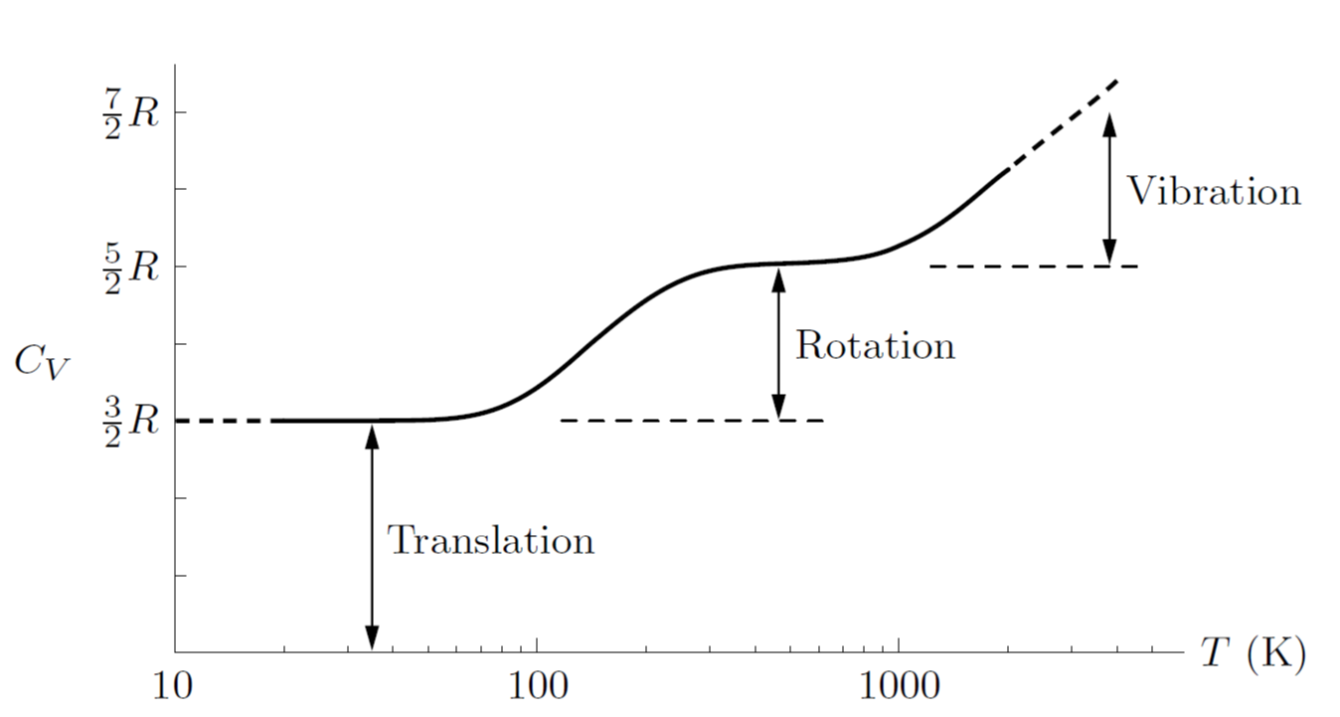
\includegraphics[width=10cm]{imgs/Cv-hydrogen.png}
\caption{Heat capacity at constant volume of one mole of hydrogen (H$_2$) gas.
Note that the temperature scale is logarithmic. }
\label{cv-h2}
\end{figure}

\begin{figure}[h]
\centering
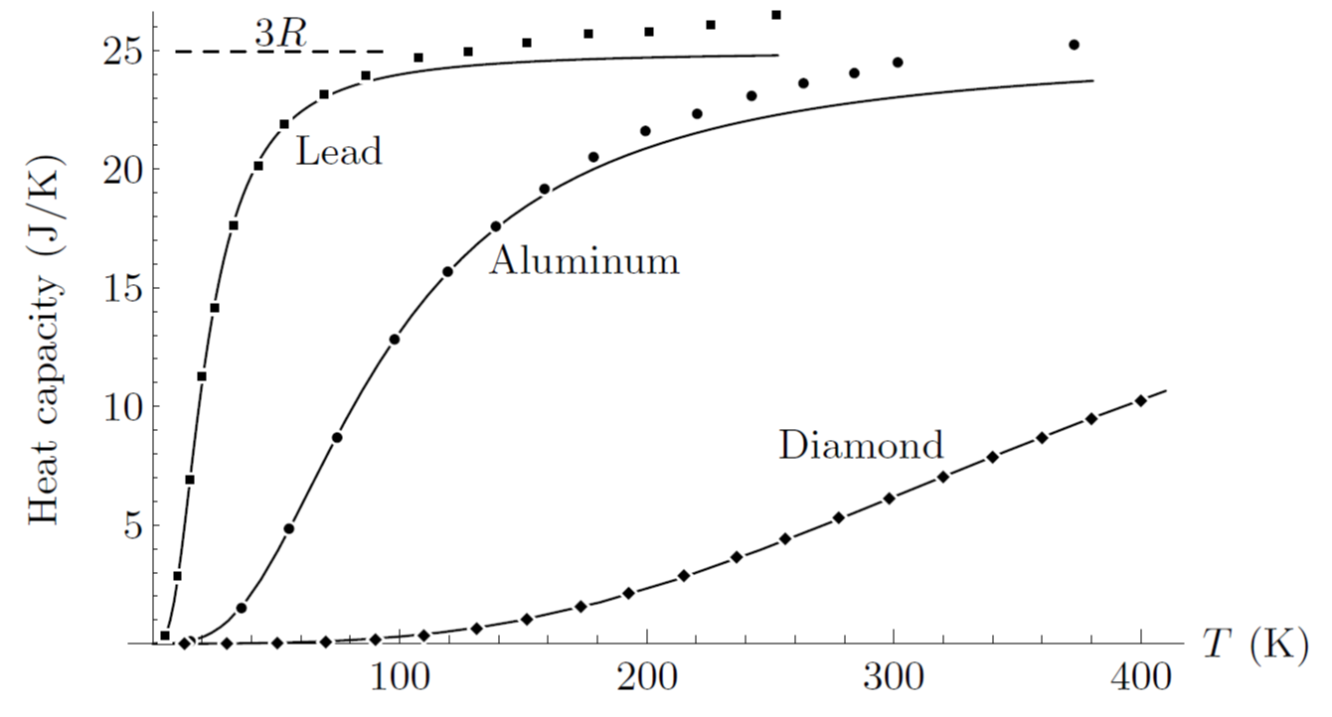
\includegraphics[width=10cm]{imgs/Cv-metal.png}
\caption{Measured heat capacities at constant pressure (data points) for
one mole each of three different elemental solids. }
\label{cv-metal}
\end{figure}

{\bf Exercises}\\
(Problem 1.44): Look up the table of thermodynamic data at room temperature. Browse through the $C_P$ values in this table, and understand them according to the equipartition theorem.\\
\begin{tabular}{|c | c | c | c |}
\hline
Type    & Examples ~~~~~~~~~~~~~~~& Ideal Value ~~& Anomaly~~~~~~~~~~~~~~~~~~~ \\\hline
monoatomic gas  &   &   &   \\\hline
diatomic gas    &   &   &   \\\hline
polyatomic(linear) gas &   &   &   \\\hline
polyatomic gas &   &   &   \\\hline
Elemental solid &   &   &   \\\hline
Binary solid &   &   &   \\\hline

\end{tabular}\\\\


\section{Enthalpy}
Constant pressure processes occur quite often in chemical reactions and phase transformations. Keeping track of the work done during these processes gets to be a pain. Any idea to make it more convenient? Instead of talking about the energy, we can agree to add the work due to $PV$ in the given environment. This results in a new quantity called the enthalpy ($H$),
\begin{equation} H = U + PV \end{equation}
Conveniently, we can express 
\begin{equation} C_P = \bigg (\frac {\partial H}{\partial T} \bigg)_{P}.
\end{equation}
Think about
\begin{enumerate}
\item{diamond and graphite under high pressure}
\item{formation enthalpy of H$_2$ and O$_2$ gas combine to water}
\end{enumerate}

